\documentclass[conference]{IEEEtran}

% correct bad hyphenation here
\hyphenation{op-tical net-works semi-conduc-tor}

\usepackage{graphicx}

% on table
\usepackage{array}

% on equasion
\usepackage[only,varodot]{stmaryrd}
\usepackage[euler]{textgreek}
\usepackage{MnSymbol}

\graphicspath{{./img/}}


\begin{document}

\title{Report 1}

\author{
	\IEEEauthorblockN{Jun Huang}
	\IEEEauthorblockA{
		Gina Cody School of Engineering and Computer Science\\
		Concordia University\\
		Email: youyinnn@foxmail.com
	}
}
\maketitle

\begin{abstract}
	The abstract goes here.
\end{abstract}

\begin{IEEEkeywords}
	1-bit Adder, Hybird Adder, CMOS,
\end{IEEEkeywords}

\section{Introduction}

...

An XOR-XNOR-based hybrid full adder design has been proposed\cite{20212210429416}
which uses an XOR-XNOR module combined with the carry-generation module and the sum-generation module.
As the designers discussed, it is a scalable and full-swing FA
with some performance improvements compared with several existing state-of-the-art FAs.

in section 2, xxx will be discussed...

% 列举其他找到的设计 但是并不在报告里讨论 因为设计的论文本身提供的信息在不做模拟的情况下难以放在同一个标准下进行比较 或者论文本身缺失了参数信息

\section{FA-1: XOR-XNOR-based Hybrid Full Adder}

\subsection{Design}

The FA-1\cite{20212210429416} design contains three modules to perform a 1-bit full adder operation.
Firstly, an XOR-XNOR circuit will take original inputs \(A\) and \(B\) as its input and produce two signals,
one is from the XNOR gate marked as \(S_{xnor\_out}\) and the other is from the XOR gate marked as \( S_{xor\_out}\).
Then, a TG-based circuit as the second module will take both signal and the input carry \(C_{in}\) to calculate the \(Sum\)
while a third module will then use the \(C_{in}\) along with \(A\), \(B\) and signals \(S_{xnor\_out}\), \( S_{xor\_out}\) to generate the carry \(C_{out}\).

Fig. \ref{fig:fa1-bd} presents the block diagram of the design.

\begin{figure}[!ht]
	\centering
	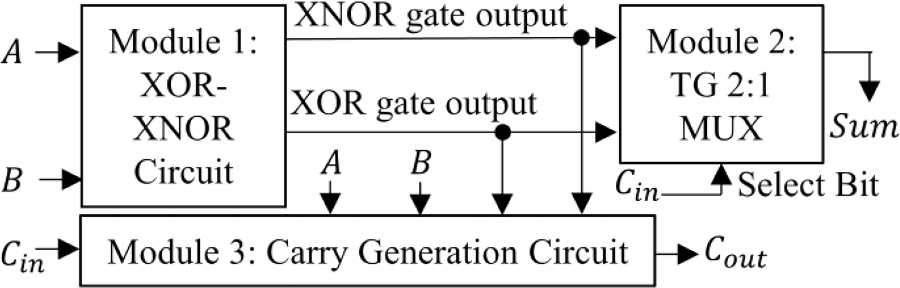
\includegraphics[width=2.7in]{fa1-block diagram.png}
	\caption{Block Diagram Of FA-1}
	\label{fig:fa1-bd}
\end{figure}

\subsubsection{Module 1}XOR-XNOR Circuit Design

The circuit consists of 10 transistors as is shown in Fig. \ref{fig:fa1-xor-xnor}.

\begin{figure}[!ht]
	\centering
	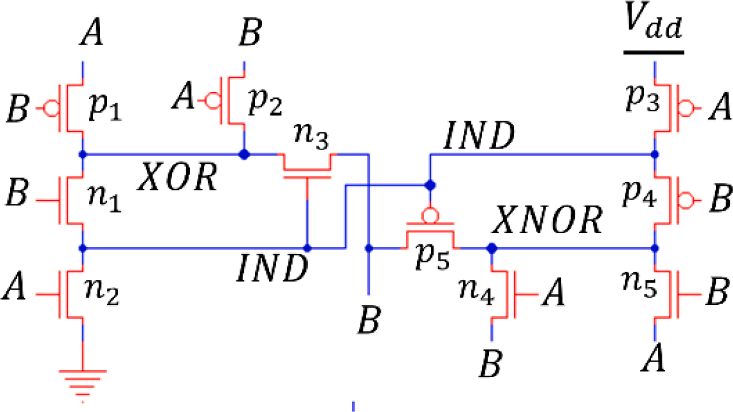
\includegraphics[width=2.2in]{fa1-xor-xnor circuit.png}
	\caption{XOR-XNOR Circuit}
	\label{fig:fa1-xor-xnor}
\end{figure}

For all the possible \(A\), \(B\) inputs,
table \ref{tb:xor-xnor} presents all the output patterns also the responsible transistors within the circuit.
As the table presented, it is clear that at least one transistor path can provide full swing output to prevent threshold voltage loss.

\begin{table*}[!htb]
	\renewcommand{\arraystretch}{1.3}
	\caption{Operation Table of the XOR-XNOR circuit}
	\centering
	\begin{tabular}{p{1.5cm}p{1.5cm}p{1.5cm}p{4cm}p{4cm}l}
		\hline
		\multicolumn{6}{ c }{\bfseries XOR Circuit}                                                                                                                                                                                     \\
		\multicolumn{3}{ c }{\bfseries Input} & \multicolumn{2}{ c }{\bfseries Output Transistor Path} & \multicolumn{1}{ c }{\bfseries Output}                                                                                         \\
		Pattern no.                           & \(A\)                                                  & \(B\)                                  & Full Swing Transistor Path & Non-Full Swing Transistor Path & Output Signal\(/\)logic \\
		\hline
		1.                                    & 0                                                      & 0                                      & \(n_3\)                    & \(p_1/p_2\)                    & \(B/0\)                 \\
		2.                                    & 0                                                      & 1                                      & \(p_2\)                    & \(n_1/n_3\)                    & \(B/1\)                 \\
		3.                                    & 1                                                      & 0                                      & \(p_1\)                    & None                           & \(A/1\)                 \\
		4.                                    & 1                                                      & 0                                      & \(n_1\) and \(n_2\)        & None                           & \(0\)                   \\
		\hline
		\multicolumn{6}{ c }{\bfseries XNOR Circuit}                                                                                                                                                                                    \\
		\multicolumn{3}{ c }{\bfseries Input} & \multicolumn{2}{ c }{\bfseries Output Transistor Path} & \multicolumn{1}{ c }{\bfseries Output}                                                                                         \\
		Pattern no.                           & \(A\)                                                  & \(B\)                                  & Full Swing Transistor Path & Non-Full Swing Transistor Path & Output Signal\(/\)logic \\
		\hline
		1.                                    & 0                                                      & 0                                      & \(p_3\) and \(p_4\)        & None                           & \(1\)                   \\
		2.                                    & 0                                                      & 1                                      & \(n_5\)                    & None                           & \(A/0\)                 \\
		3.                                    & 1                                                      & 0                                      & \(n_4\)                    & \(p_4/p_5\)                    & \(B/0\)                 \\
		4.                                    & 1                                                      & 0                                      & \(p_5\)                    & \(n_4/n_5\)                    & \(B/1\)                 \\
		\hline
	\end{tabular}
	\label{tb:xor-xnor}
\end{table*}

\subsubsection{Module 2}Sum Generation Circuit

From the Table \ref{tb:fa-tf}, two paths for the \(Sum\) generation can be concluded:

when \(C_{in} = 0\):
\[
	Sum = A \oplus B
\]

when \(C_{in} = 1\):
\[
	Sum = A \varodot B
\]

\begin{table}[!ht]
	\renewcommand{\arraystretch}{1.3}
	\caption{True-False Table of FA}
	\centering
	\begin{tabular}{p{1cm}p{1cm}p{1cm}p{1cm}p{1cm}}
		\hline
		\multicolumn{3}{ c }{\bfseries Inputs} & \multicolumn{2}{ c }{\bfseries Outputs}                                 \\
		\(C_{in}\)                             & \(A\)                                   & \(B\) & \(C_{out}\) & \(Sum\) \\
		\hline
		0                                      & 0                                       & 0     & 0           & 0       \\
		                                       & 0                                       & 1     & 0           & 1       \\
		                                       & 1                                       & 0     & 0           & 1       \\
		                                       & 1                                       & 1     & 1           & 0       \\
		1                                      & 0                                       & 0     & 0           & 1       \\
		                                       & 0                                       & 1     & 1           & 0       \\
		                                       & 1                                       & 0     & 1           & 0       \\
		                                       & 1                                       & 1     & 1           & 1       \\
		\hline
	\end{tabular}
	\label{tb:fa-tf}
\end{table}

For input selection, a 2:1 Multiplexer(2:1 MUX) based on Transmission Gate(TG) has been used for the \(Sum\) generation.

As is given in Fig. \ref{fig:fa1-circuit}, two TGs are used for implementing 2:1 MUX logic and with this manner,
the \(Sum\) generation circuit can also provide full swing output.

\begin{figure}[!ht]
	\centering
	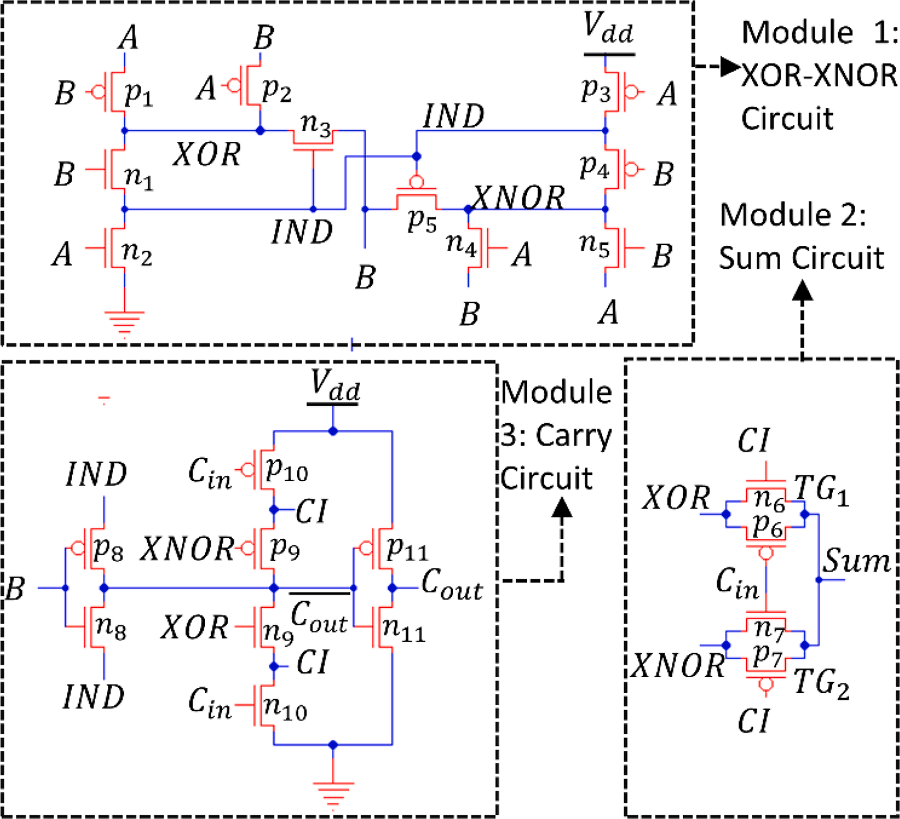
\includegraphics[width=2.7in]{fa1-circuit.png}
	\caption{FA-1 Circuit}
	\label{fig:fa1-circuit}
\end{figure}

\subsubsection{Module 3}Carry Generation Circuit

As per Fig. \ref{fig:fa1-circuit}, the \(Carry\) generation circuit uses a CCMOS logic-based inverter at the output.
With this logic, the output voltage level of this circuit is either \(V_{dd}\) or \(G_{nd}\) level.
It is a good design for the extensibility of the circuit
since the design of the carry generation logic is the most important factor of the scalability of the wide word length adders.


\subsection{Discussion}

FA-1 shows impressive improvements compared to many other FAs.
The presenters are intended to solve the voltage degradation issue with the hybrid logic-based design,
hence they design the XOR-XNOR-based circuit to produce full swing output for its next stage
and choose TG for implementing the sum generation circuit.

Finally, for the purpose of high-speed calculations and good scalabilities,
they apply the CCMOS technique at the output terminial.
The designed carry generation circuit can be extended to multiple bits adder structures with no additional voltage level restoring buffers.
Furthermore, this logic can reduce the carry chain delay with involving just one pull-up and pull-down transistors.

As for the area overhead, a total of 22 transistors are used to produce this FA, namely, 10 on module one, 4 on module 2, and 8 on module 3.

According to the presenters' simulation using 45nm technique and 1 voltage supply, compare with the conventional CMOS FA\cite{weste2015cmos} and other recent FA designs\cite{9068497,18743001},
% this design has 19.35\% improvement in Silicon area, 33.59\% improvement in Average Power, 36.15\% improvement in Propagation Delay, 56.22\% improvement in Area Delay Product, and 57.59\% improvement in Power Delay Product.
this design achieves many improvements which can be shown in the Table \ref{tb:fa1-comparison}.

\begin{table*}[!ht]
	\renewcommand{\arraystretch}{1.3}
	\caption{FA Performance Investigation Performed By }
	\centering
	\begin{tabular}{l c l l l l l l l l l l}
		\hline
		\bfseries FA Design            & \bfseries TC & \multicolumn{5}{ c }{\bfseries Performance} & \multicolumn{5}{ c }{\bfseries Improvements with Respect to CCMOS FA}                                                                                                                                                                  \\
		                               &              & Area(\textmugreek\(m^2\))                   & AP(\textmugreek\(W\))                                                 & PD(ps)         & ADP(\textmugreek\(m^2\).ps) & PDP(\textalpha J) & Area($\slashdiv$) & AP($\slashdiv$) & PD($\slashdiv$) & ADP($\slashdiv$) & PDP($\slashdiv$) \\
		\hline
		CCMOS\cite{weste2015cmos}      & 28           & 10.13                                       & 1.28                                                                  & 60.3           & 610.84                      & 77.18             & 0.00              & 0.00            & 0.00            & 0.00             & 0.00             \\
		Kandpal's\cite{9068497}        & 20           & 9.18                                        & 0.92                                                                  & 54.06          & 496.27                      & 49.74             & 9.38              & 28.13           & 10.35           & 18.76            & 35.55            \\
		Sanapala's\cite{18743001}      & 14           & \bfseries 7.38                              & 0.75                                                                  & 56.7           & 415.45                      & 42.53             & \bfseries 27.15   & \bfseries 41.41 & 5.97            & 31.99            & 44.90            \\
		Presented\cite{20212210429416} & 22           & 8.17                                        & 0.85                                                                  & \bfseries 38.5 & \bfseries 267.40            & \bfseries 32.73   & 19.35             & 33.59           & \bfseries 36.15 & \bfseries 56.22  & \bfseries 57.59  \\
		\hline
	\end{tabular}
	\label{tb:fa1-comparison}
\end{table*}

\section{Design B}

An XOR-XNOR-based hybrid full adder design has been proposed\cite{20212210429416}
which uses an XOR-XNOR module combined with the carry-generation module and the sum-generation module.
As the designers discussed, it is a scalable and full-swing FA
with some performance improvements compared with several existing state-of-the-art FAs.An XOR-XNOR-based hybrid full adder design has been proposed\cite{20212210429416}
which uses an XOR-XNOR module combined with the carry-generation module and the sum-generation module.
As the designers discussed, it is a scalable and full-swing FA
with some performance improvements compared with several existing state-of-the-art FAs.

\section{Design C}

An XOR-XNOR-based hybrid full adder design has been proposed\cite{20212210429416}
which uses an XOR-XNOR module combined with the carry-generation module and the sum-generation module.
As the designers discussed, it is a scalable and full-swing FA
with some performance improvements compared with several existing state-of-the-art FAs.An XOR-XNOR-based hybrid full adder design has been proposed\cite{20212210429416}
which uses an XOR-XNOR module combined with the carry-generation module and the sum-generation module.
As the designers discussed, it is a scalable and full-swing FA
with some performance improvements compared with several existing state-of-the-art FAs.

\section{Design D}

An XOR-XNOR-based hybrid full adder design has been proposed\cite{20212210429416}
which uses an XOR-XNOR module combined with the carry-generation module and the sum-generation module.
As the designers discussed, it is a scalable and full-swing FA
with some performance improvements compared with several existing state-of-the-art FAs.An XOR-XNOR-based hybrid full adder design has been proposed\cite{20212210429416}
which uses an XOR-XNOR module combined with the carry-generation module and the sum-generation module.
As the designers discussed, it is a scalable and full-swing FA
with some performance improvements compared with several existing state-of-the-art FAs.

\section{Comparison}

An XOR-XNOR-based hybrid full adder design has been proposed\cite{20212210429416}
which uses an XOR-XNOR module combined with the carry-generation module and the sum-generation module.
As the designers discussed, it is a scalable and full-swing FA
with some performance improvements compared with several existing state-of-the-art FAs.An XOR-XNOR-based hybrid full adder design has been proposed\cite{20212210429416}
which uses an XOR-XNOR module combined with the carry-generation module and the sum-generation module.
As the designers discussed, it is a scalable and full-swing FA
with some performance improvements compared with several existing state-of-the-art FAs.

\section{Conclusion}

An XOR-XNOR-based hybrid full adder design has been proposed\cite{20212210429416}
which uses an XOR-XNOR module combined with the carry-generation module and the sum-generation module.
As the designers discussed, it is a scalable and full-swing FA
with some performance improvements compared with several existing state-of-the-art FAs.An XOR-XNOR-based hybrid full adder design has been proposed\cite{20212210429416}
which uses an XOR-XNOR module combined with the carry-generation module and the sum-generation module.
As the designers discussed, it is a scalable and full-swing FA
with some performance improvements compared with several existing state-of-the-art FAs.

\bibliographystyle{ieeetr}
\bibliography{bibliographies}
\end{document}
